\chapter{Implementation - Computer Vision}

This chapter will cover the implementation methods on computer vision side of this project using either ASUS Xtion or ZED Mini. By adjusting some settings which will be discussed in this chapter, the algorithm works for both cameras. The entire code for this part can be seen in !!!!!!!!!!

\section{Camera Setup}
The dependency package allow specific camera to communicate with ROS is shown in Table \ref{camerapackage}, which contains corresponding launch files. Entering the launch command in the terminal can start the package driver. After that, a list of camera topics including RGB, depth, and point-clouds etc can be subscribed for further processing. 

\begin{table}[H]
\centering
\resizebox{\columnwidth}{!}{
\begin{tabular}{||c||c|c||}
\hline
Camera & Dependency package & Launch command \\ \hline \hline
ASUS Xtion & $openni2$ & $roslaunch$ $openni2\_launch$ $openni2.launch$ \\ \hline
ZED Mini & $zed-ros-wrapper$ & $roslaunch$ $zed\_wrapper$ $zedm.launch$ \\ \hline
\end{tabular}
}
\caption{The dependency packages and launch commands for Cameras}
\label{camerapackage}
\end{table}

In ROS, video streams are represented by these sequences of images. If user would like to use ROS images in conjunction with OpenCV, $CvBridge$ package provides the converting interface, which is used in this project as well.

\begin{figure}[H]
\centering
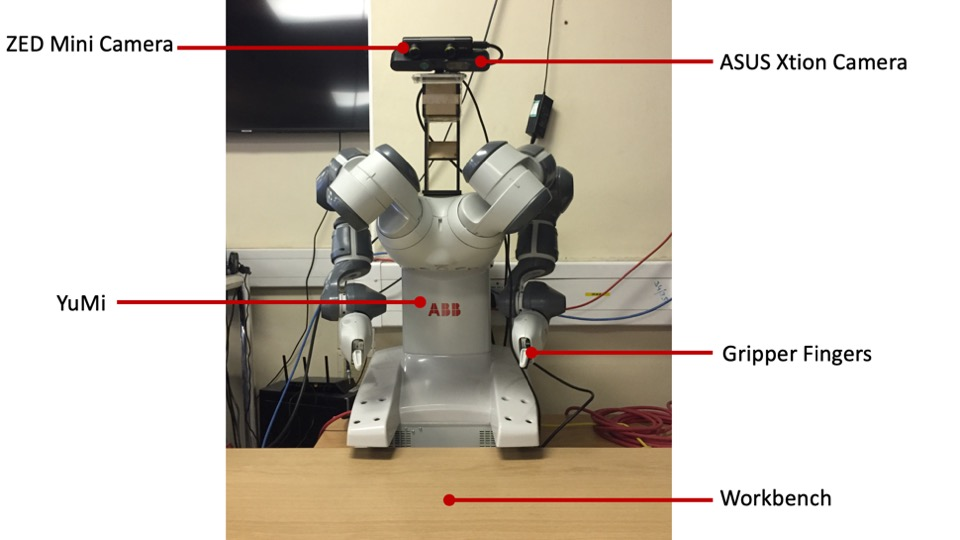
\includegraphics[width = \columnwidth]{Implementation/cv/yumicamera.jpg}
\caption{YuMi and ASUS Xtion camera position setup}
\label{5.1}
\end{figure}

Figure \ref{5.1} displays the relative position between YuMi and the two cameras. The cameras' location and orientation transform from YuMi frame $yumi\_base\_link$ are illustrated in Table \ref{cameraframeset} and written in the YuMi launch file (see !!!!!!!). These data are measured manually, which allow ROS $TF$ to perform frame transformation between any camera detected objects and YuMi in this project. 
\begin{table}[H]
\centering
\resizebox{\columnwidth}{!}{
\begin{tabular}{||c||c|c||}
\hline
Camera & Camera frame & Transform from $yumi\_base\_link$ \\ \hline\hline
ASUS Xtion & /camera\_link & {[}0.2013, 0.0641, 0.6934, -0.0238, 0.4836, -0.0141, 0.875{]} \\ \hline
ZED Mini & /zed\_left\_camera\_frame & {[}0.2263, 0.0541, 0.7134, -0.0238, 0.4836, -0.0141, 0.875{]} \\ \hline
\end{tabular}
}
\caption{Transform settings between YuMi and cameras}
\label{cameraframeset}
\end{table}

\section{Shoe Detection} \label{shoedetection}
As mentioned in Background Chapter, YOLO9000 will be used for shoe detection. \citep{bjelonicYolo2018} developed the YOLO ROS interface called $darknet\_ros$, which supports using YOLO on both CPU and GPU. This package depends on OpenCV, boost (C++ library) and CUDA (if use Nvidia GPU for faster processing). Detailed installation and setup instructions can be found in User Guide Chapter. 

\begin{figure}[H]
\centering
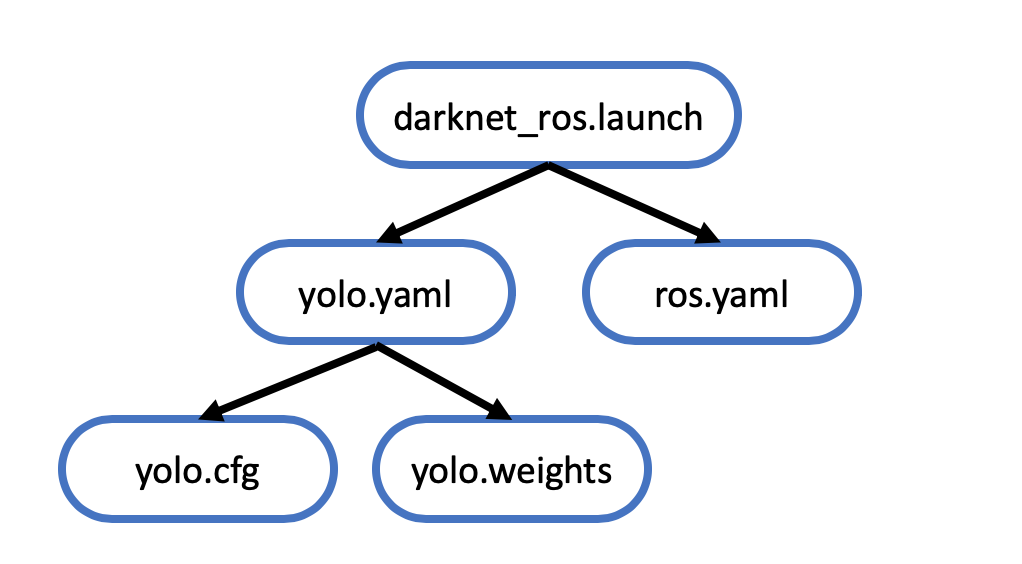
\includegraphics[width = 0.6\columnwidth]{Implementation/cv/yolofile.png}
\caption{Important files in YOLO package}
\label{yolofolder}
\end{figure}

Figure \ref{yolofolder} shows some important files in $darknet\_ros$. The $.weights$ file and $.cfg$ file contain the trained weights and labels etc for a specific YOLO version. Here, I use YOLO9000. The $yolo.yaml$ file points to these two files and defines a threshold value $0.3$. The results will be reported only if the YOLO9000 prediction probability of a detection class exceeds this value. 

The file named $ros.yaml$ defines the names and some parameters of the publishers, subscribers and actions of $darknet\_ros.launch$. Here, the input can be set as camera topic $/camera/rgb/image\_raw$ for ASUS Xtion, or $/zed\slash zed\_node\slash rgb\slash image\_rect\_color$ for ZED Mini, both contain the RGB images taken by the camera. It publishes several topics but only $/darknet\_ros/bounding\_boxes$ will be used in the following algorithms. The messages in this topic include the prediction class names of objects, their prediction probabilities and 2D bounding box coordinates ($xmin$, $xmax$, $ymin$, and $ymax$). If the category is predicted as 'shoe' or 'footwear', the corresponding box coordinates will be recorded. By speeding up with GPU, $darknet\_ros$ can update the detection results approximately every 0.05 seconds.

\begin{figure}[H]
\centering
\subfigure[RGB image]{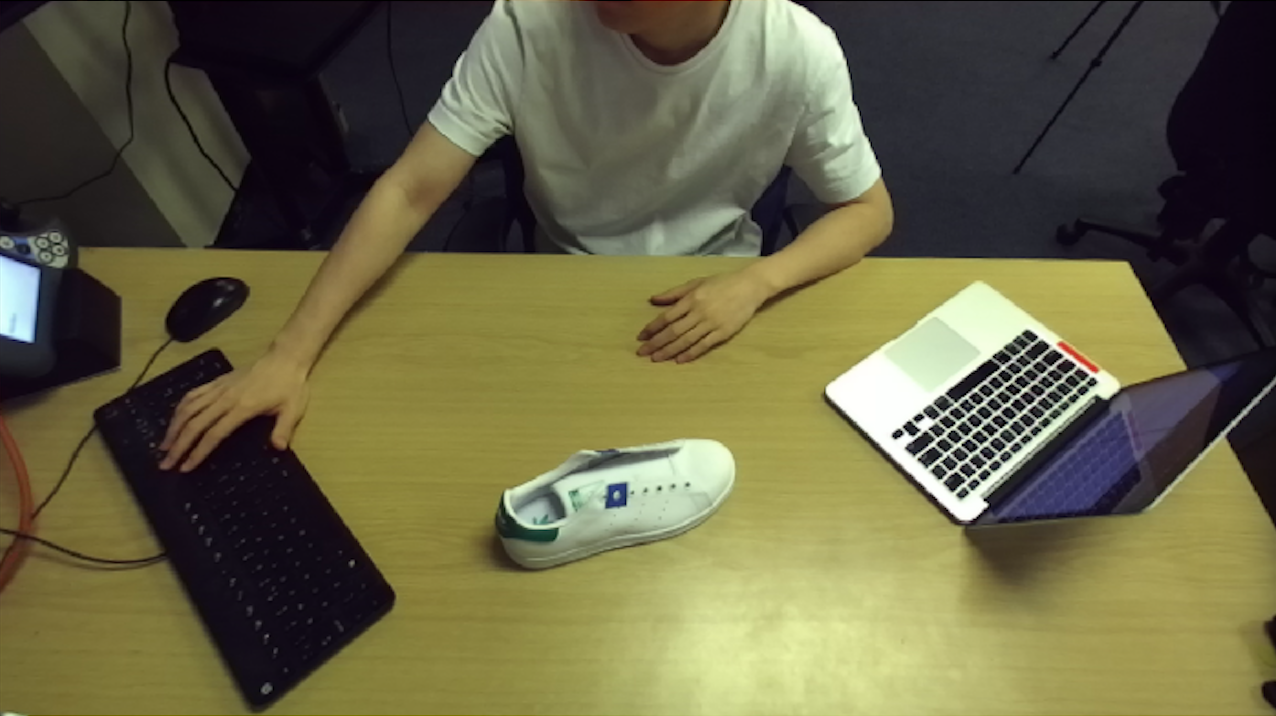
\includegraphics[width = 0.45\columnwidth]{Implementation/cv/zedrgb.png}}
\subfigure[YOLO detection image including bounding boxes]{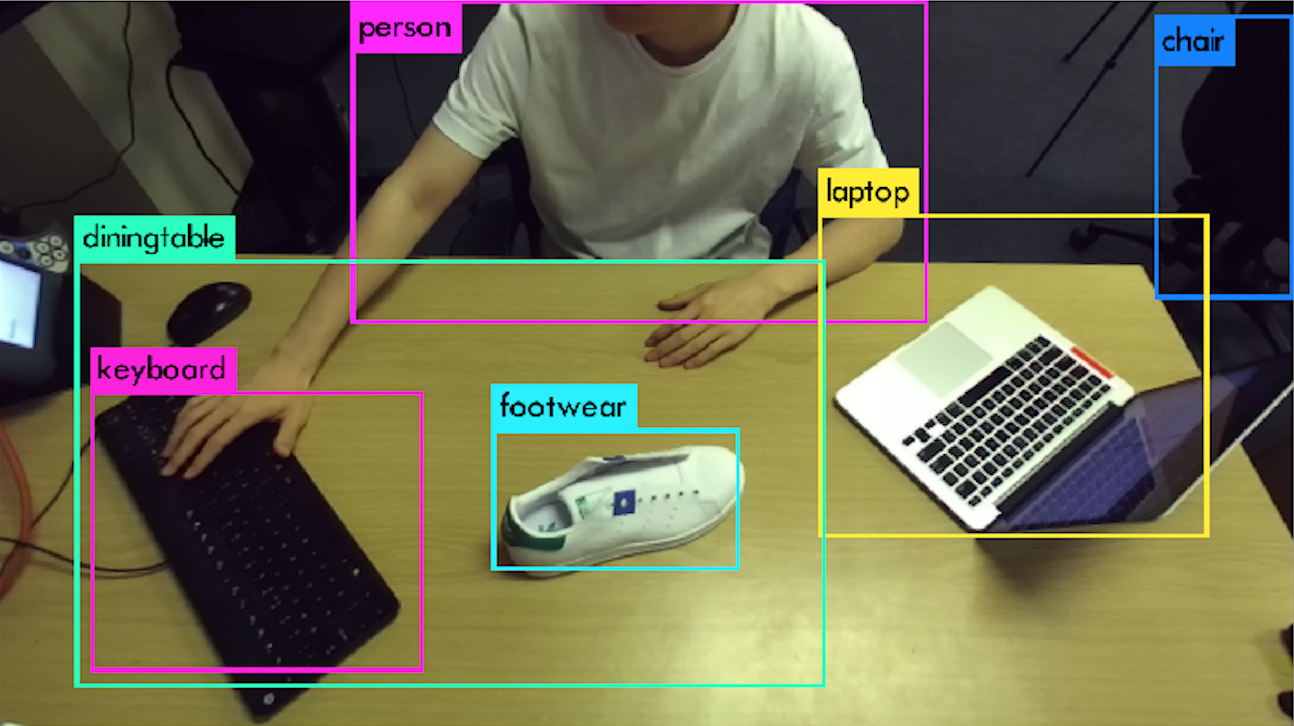
\includegraphics[width = 0.45\columnwidth]{Implementation/cv/zedyolo.png}}
\caption{ZED Mini camera image before and after using YOLO detection system}
\label{5.2zed}
\end{figure}

\begin{figure}[H]
\centering
\subfigure[RGB raw image]{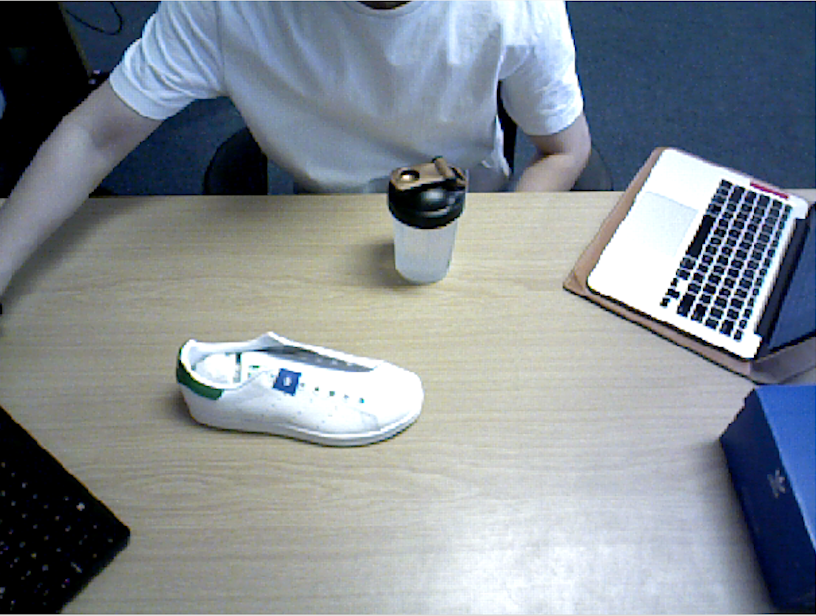
\includegraphics[width = 0.45\columnwidth]{Implementation/cv/raw.png}}
\subfigure[YOLO detection image including bounding boxes]{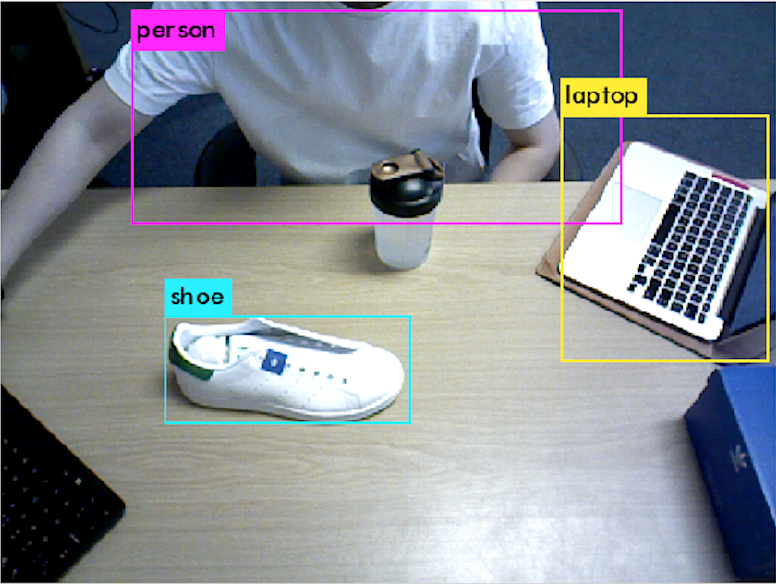
\includegraphics[width = 0.45\columnwidth]{Implementation/cv/yolo.png}}
\caption{ASUS Xtion camera image before and after using YOLO detection system}
\label{5.2asus}
\end{figure}

Figure \ref{5.2zed} and \ref{5.2asus} are the examples of YOLO detection using different cameras.



\section{Required Locations for Shoe Pose Adjustment} \label{shoeadjust}

\begin{figure}[H]
\centering
\subfigure[]{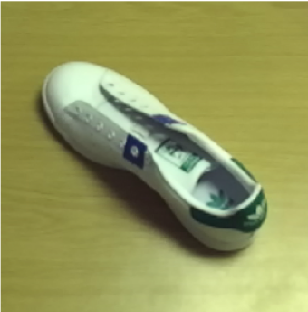
\includegraphics[width = 0.15\columnwidth]{Implementation/cv/1.png}}
\subfigure[]{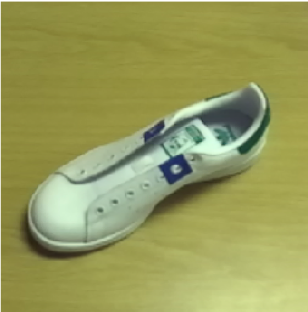
\includegraphics[width = 0.15\columnwidth]{Implementation/cv/2.png}}
\subfigure[]{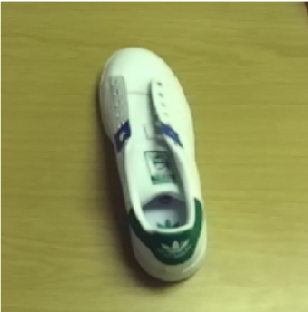
\includegraphics[width = 0.15\columnwidth]{Implementation/cv/3.png} \label{ver1}}
\subfigure[]{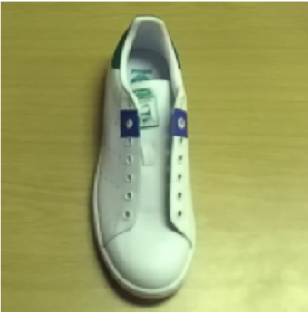
\includegraphics[width = 0.15\columnwidth]{Implementation/cv/4.png} \label{ver2}}
\subfigure[]{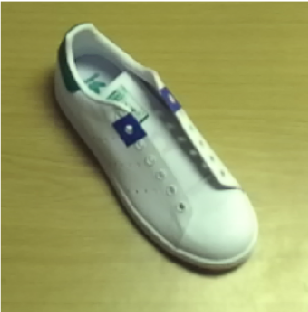
\includegraphics[width = 0.15\columnwidth]{Implementation/cv/5.png}}
\subfigure[]{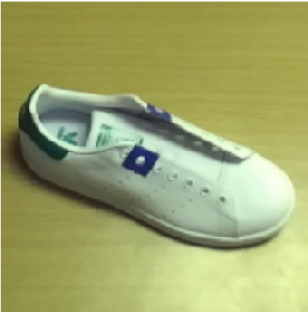
\includegraphics[width = 0.15\columnwidth]{Implementation/cv/6.png}}
\caption{Examples of possible shoe orientations}
\end{figure}

In the beginning, the shoe can be placed on the workbench in different directions, making the real manipulation difficult in some cases, especially when it is vertically placed (Figure \ref{ver1} and \ref{ver2}). Therefore, under this circumstance, its orientation need to be adjusted. Figure \ref{adjustmentidea} displays the idea. Starting at two blue points ($adl$ and $adr$), both of YuMi's grippers will move towards the orange points ($adll$ and $adrr$) simultaneously to perform the adjustment. After that, they will follow the previous paths and return to blue points in order to avoid potential collisions with the shoe. The ideal shoe pose after adjustment is shown on the right hand side.

\begin{figure}[H]
\centering
\subfigure[Before adjustment]{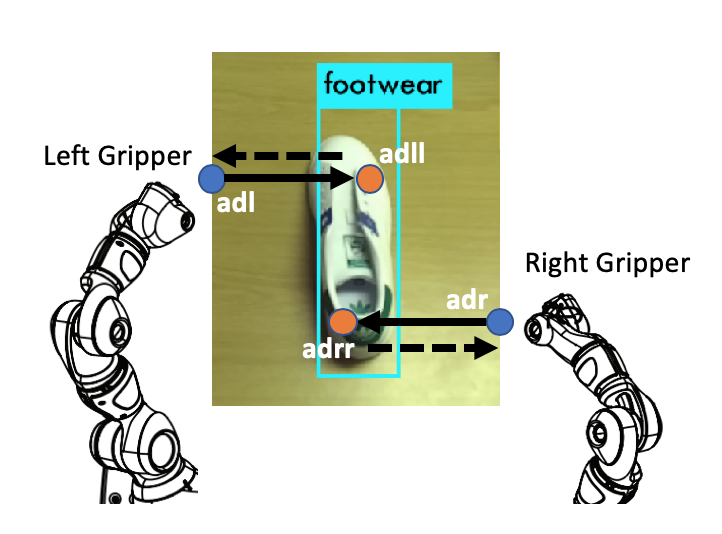
\includegraphics[width = 0.49\columnwidth]{Implementation/cv/adjustmentidea.png}}
\subfigure[After Adjustment]{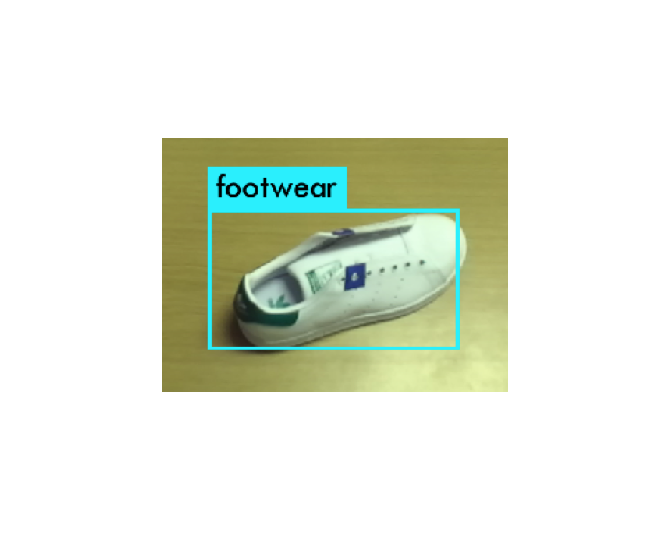
\includegraphics[width = 0.49\columnwidth]{Implementation/cv/adjustmentidea2.png}}
\caption{The shoe pose adjustment idea}
\label{adjustmentidea}
\end{figure}

To achieve this, the 2D pixel coordinates of these blue and orange points will firstly be documented, which can be determined based on the YOLO bounding box. However, YuMi still needs to know the real-world 3D locations of these points in order to move its grippers to the correct places. This can be computed by looking at the camera registered point cloud topic, which is shown in Figure \ref{ptcloud}. For ASUS Xtion, the topic name is $/camera/depth\_registered/points$. While ZED Mini uses $/zed\slash zed\_node\slash point\_cloud\slash cloud\_registered$.

\begin{figure}[H]
\centering
\subfigure[RGB raw image]{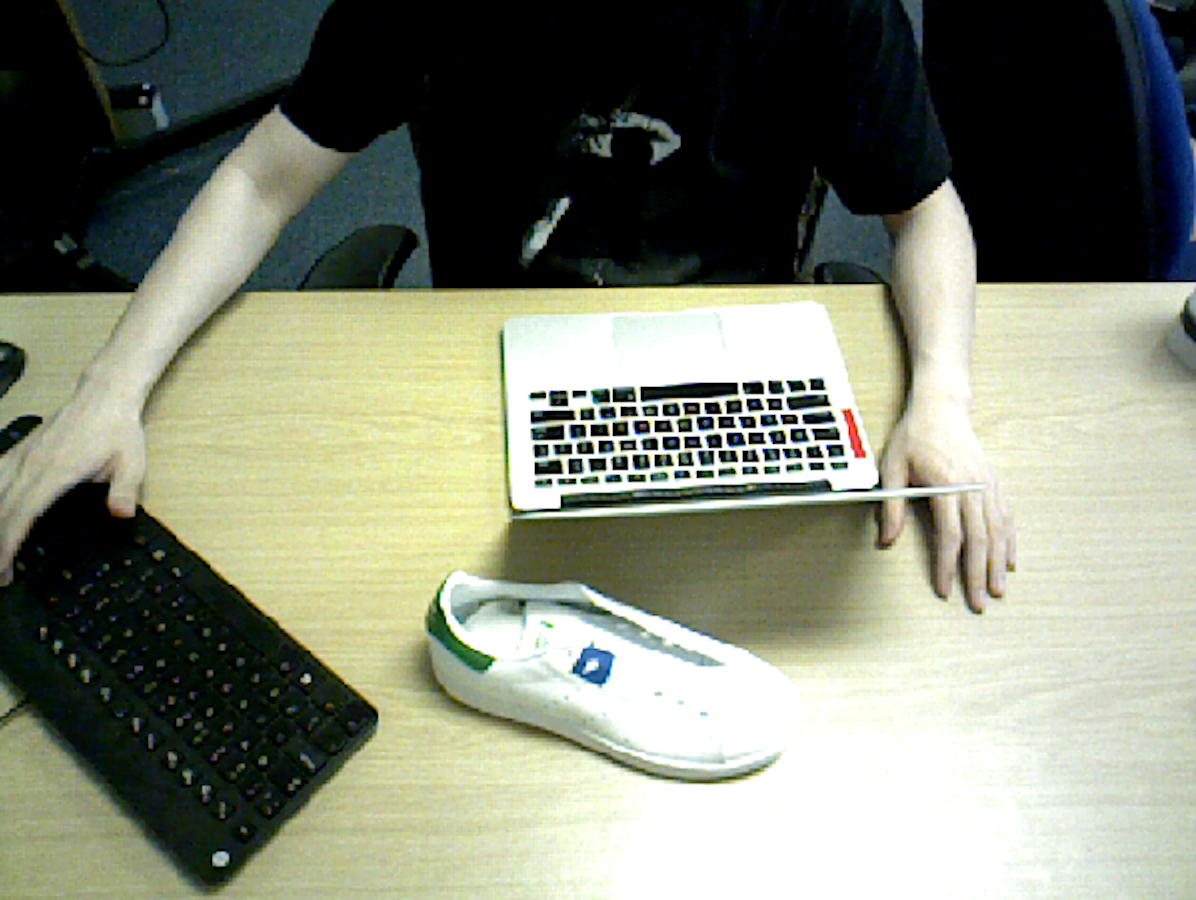
\includegraphics[width = 0.45\columnwidth, height=50mm]{Implementation/cv/rgbpt.png}}
\subfigure[Depth registered point clouds]{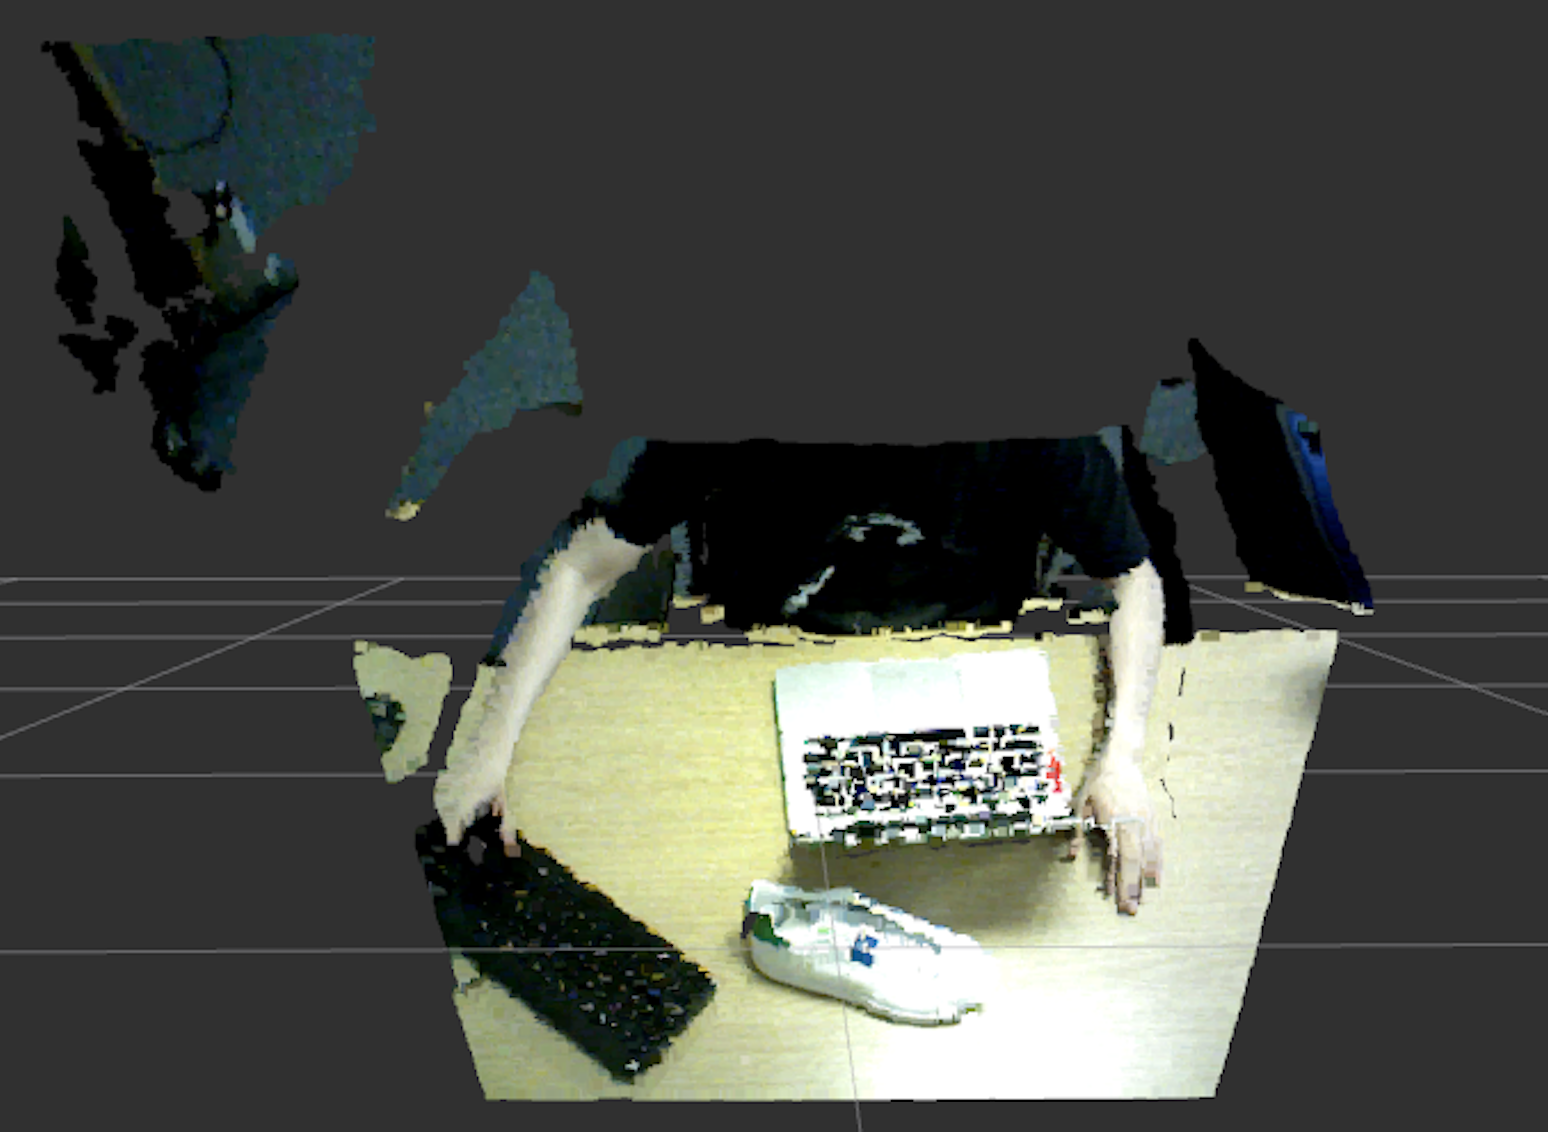
\includegraphics[width = 0.45\columnwidth, height=50mm]{Implementation/cv/ptcloud.png} \label{ptcloud}}
\caption{Messages of different ASUS Xtion camera topics}
\end{figure}

Each point cloud contains the real-world $xyz$ readings relative to the camera and RGB information. Take ASUS Xtion for example, since its image resolution is $640 \times 480$, there are total $307200$ points for each image. Sometimes, the $xyz$ readings of some points might be $nan$, which are not reliable and should be ignored. Using those 2D pixel positions calculated previously, $pc2.read\_points$ function helps find the corresponding point cloud and return the reading.

\begin{minted}[frame=single, framesep=1.5mm, baselinestretch=1, fontsize=\footnotesize, linenos, breaklines]{python}
adr = list(pc2.read_points(data, field_names = ('x', 'y', 'z'), skip_nans = True, uvs = [(self.adr_x, self.adr_y)]))
if len(adr) > 0:
    adr_x, adr_y, adr_z = adr[0]
    adr = [adr_z, -adr_x, -adr_y] #if using ASUS Xtion
    #adr = [adr_x, adr_y, adr_z] #if using ZED Mini
    self._tfpub.sendTransform((adr), tf.transformations.quaternion_from_euler(0, 0, 0), rospy.Time.now(), "adr", 'camera_link')
    #self._tfpub.sendTransform((adr), tf.transformations.quaternion_from_euler(0, 0, 0), rospy.Time.now(), "adr", '/zed_left_camera_frame') #if using ZED Mini
\end{minted}

The above code example is for calculating the real-word location of $adr$. The output reading of $pc2.read\_points$ is based on camera frame and camera axes. However, in order to move YuMi's arm around this location in later stages, the reading needs to be related to YuMi frame $yumi\_base\_link$ and using YuMi axes format. For ZED Mini, its axes are the same as YuMi's, so the reading format does not need to be modified (see line 5). While for ASUS Xtion, they are different and the corresponding adjustment is shown in line 4 of the code. 

As mentioned in Analysis and Design Chapter, $TF$ keeps the relationship between frames and will used for the frame conversion. The location $adr$ is firstly published using $sendTransdorm$ function, as a transform from camera frame $camera\_link$ or $zed\_left\_camera\_frame$ (see line 6 and 7). Then function $lookupTransform$ can then be used to obtained the location based on frame $yumi\_base\_link$, which will be further discussed in next Section \ref{adj} together with detailed adjustment implementation. Figure \ref{3dadj} shows these frames visualized in Rviz.

\begin{figure}[H]
\centering
\subfigure[Real-world shoe placement]{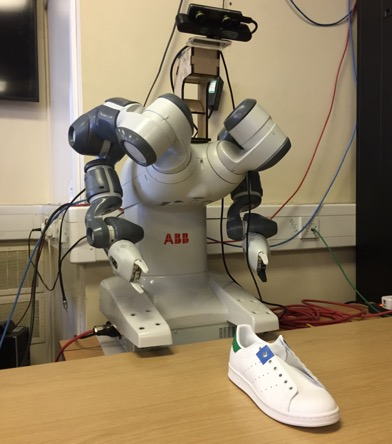
\includegraphics[height=7cm,keepaspectratio]{Implementation/cv/3dadj.jpg}}
\subfigure[The frame relationships in Rviz]{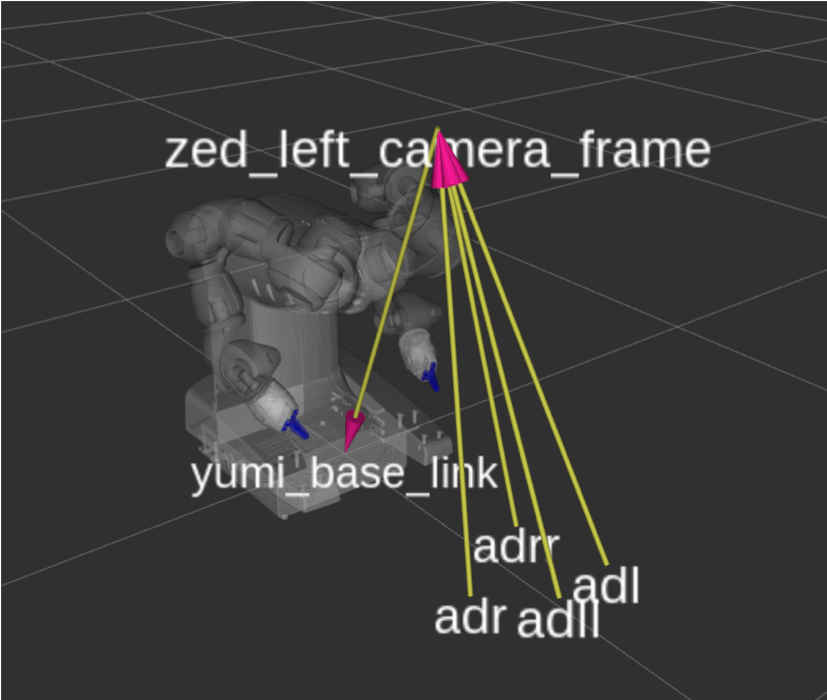
\includegraphics[height=7cm,keepaspectratio]{Implementation/cv/adjrviz.png}}
\caption{Example of required locations for shoe pose adjustment}
\label{3dadj}
\end{figure}

After adjustment, the direction of the shoe and the interested shoe hole is considered to be toward the side of the camera. Figure \ref{rangeshoe} displays the ideal range of orientations for the shoe hole after adjustment, where the red arrow represents its current orientation. In the rest of this Chapter, the orientation of the shoe hole defaults in this range.

\begin{figure}[H]
\centering
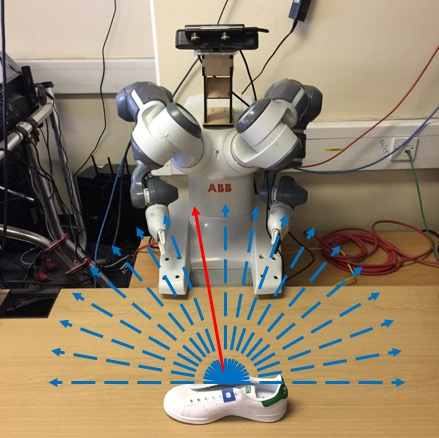
\includegraphics[width = 0.5\columnwidth]{Implementation/cv/rangetoward.jpg}
\caption{Ideal range of orientations for the shoe hole after adjustment}
\label{rangeshoe}
\end{figure}


\section{3D Location of Shoe Hole} \label{3dlocationestimation}
Since the shoe is marked, shoe hole detection can be achieved with color detection. Due to the fact that there are other objects on the workbench and color tracking is very sensitive to light condition, perform this technique using entire image cannot provide accurate results. Therefore, the image will firstly be cropped using $xmin$, $xmax$, $ymin$, and $ymax$ value computed in section \ref{shoedetection}. Color detection only applies to the cropped region of interest.

The image of shoe always contains a certain level of high frequency noise. Various blurring and smoothing techniques have been tried to tackle this issue and their results are shown in Figure \ref{zedfilter} second line. The blurred image is then converted to HSV color space. After that, a mask for color 'blue' is constructed using its predefined lower and color boundaries. The $erode$ and $dilate$ functions are then performed to remove any small blobs remain in the mask. It can be discovered that basically all the four filter can provide a reasonable mask of shoe hole area.

\begin{figure}[H]
\centering
\subfigure{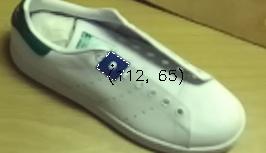
\includegraphics[width = 0.24\columnwidth]{Implementation/cv/zbi1.png}}
\subfigure{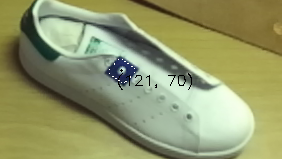
\includegraphics[width = 0.24\columnwidth]{Implementation/cv/zg1.png}}
\subfigure{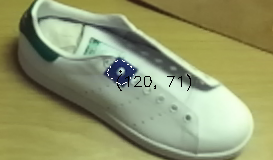
\includegraphics[width = 0.24\columnwidth]{Implementation/cv/zm1.png}}
\subfigure{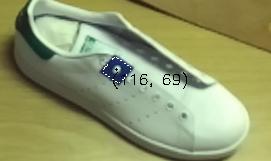
\includegraphics[width = 0.24\columnwidth]{Implementation/cv/zb1.png}}

\subfigure{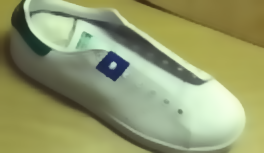
\includegraphics[width = 0.24\columnwidth]{Implementation/cv/zbi2.png}}
\subfigure{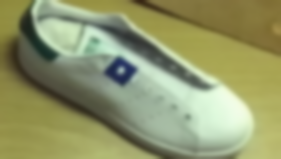
\includegraphics[width = 0.24\columnwidth]{Implementation/cv/zg2.png}}
\subfigure{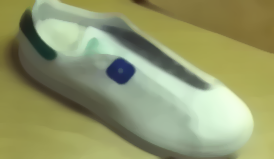
\includegraphics[width = 0.24\columnwidth]{Implementation/cv/zm2.png}}
\subfigure{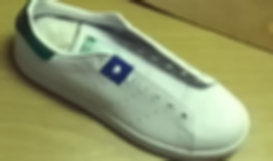
\includegraphics[width = 0.24\columnwidth]{Implementation/cv/zb2.png}}

\subfigure{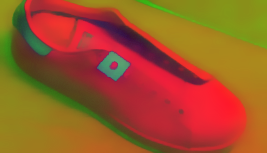
\includegraphics[width = 0.24\columnwidth]{Implementation/cv/zbi3.png}}
\subfigure{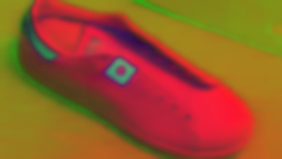
\includegraphics[width = 0.24\columnwidth]{Implementation/cv/zg3.png}}
\subfigure{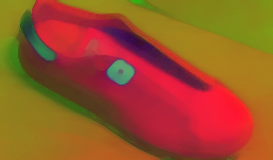
\includegraphics[width = 0.24\columnwidth]{Implementation/cv/zm3.png}}
\subfigure{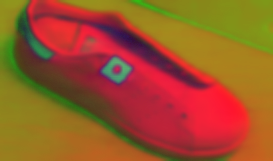
\includegraphics[width = 0.24\columnwidth]{Implementation/cv/zb3.png}}

\subfigure{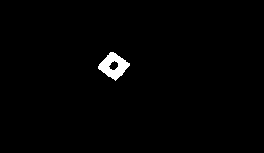
\includegraphics[width = 0.24\columnwidth]{Implementation/cv/zbi4.png}}
\subfigure{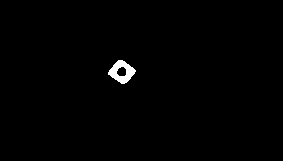
\includegraphics[width = 0.24\columnwidth]{Implementation/cv/zg4.png}}
\subfigure{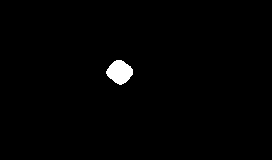
\includegraphics[width = 0.24\columnwidth]{Implementation/cv/zm4.png}}
\subfigure{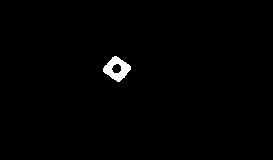
\includegraphics[width = 0.24\columnwidth]{Implementation/cv/zb4.png}}

\subfigure{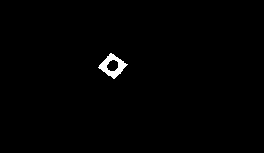
\includegraphics[width = 0.24\columnwidth]{Implementation/cv/zbi5.png}}
\subfigure{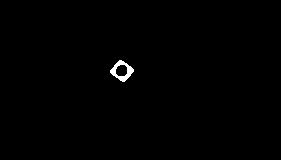
\includegraphics[width = 0.24\columnwidth]{Implementation/cv/zg5.png}}
\subfigure{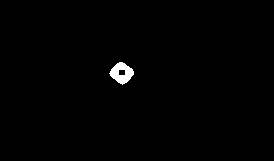
\includegraphics[width = 0.24\columnwidth]{Implementation/cv/zm5.png}}
\subfigure{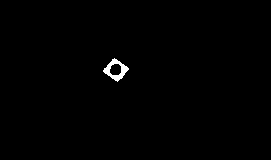
\includegraphics[width = 0.24\columnwidth]{Implementation/cv/zb5.png}}

\subfigure[Bilateral filter]{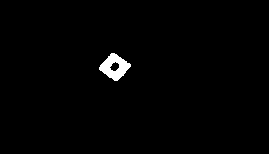
\includegraphics[width = 0.24\columnwidth]{Implementation/cv/zbi6.png}}
\subfigure[Gaussian filter]{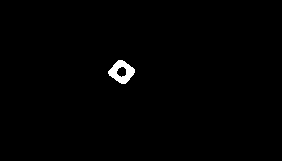
\includegraphics[width = 0.24\columnwidth]{Implementation/cv/zg6.png}}
\subfigure[Median filter]{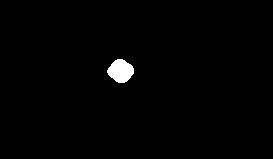
\includegraphics[width = 0.24\columnwidth]{Implementation/cv/zm6.png}}
\subfigure[Normalized Box filter]{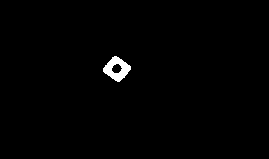
\includegraphics[width = 0.24\columnwidth]{Implementation/cv/zb6.png}}
\caption{Image processing of extracted shoe region using ZED Mini. Each column uses one specific type of blurred filter. For each column, from top to bottom, each image is, in turn, the original image labeled with detected contour area and its centroid coordinates, smoothed image after applying the linear filter, image of HSV color space of the smoothed image, mask for color 'blue', mask after $erode$ function, and the final mask after $dilate$ function}
\label{zedfilter}
\end{figure}

The contour(s) of blue area(s) are then calculated. If at least one contour is discovered, the largest one in the mask will be used and its centroid is computed accordingly. Noticed that this centroid coordinate is for the cropped image. Therefore, $xmin$ and $ymin$ must be added back to give the pixel coordinate of the original image. Finally, if the contour area lies between a predefined range, the calculated centroid will be regarded as the centroid of the shoe hole.

\begin{figure}[H]
\centering
\subfigure[Real-world shoe placement]{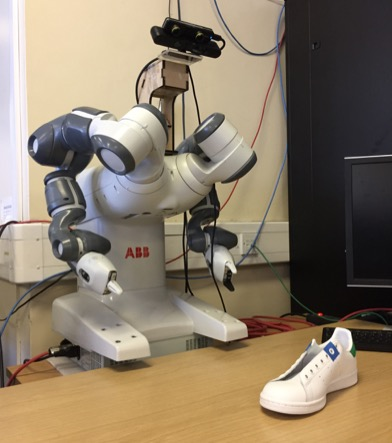
\includegraphics[height=7cm,keepaspectratio]{Implementation/cv/3dposw.jpg}}
\subfigure[The frame relationships in Rviz]{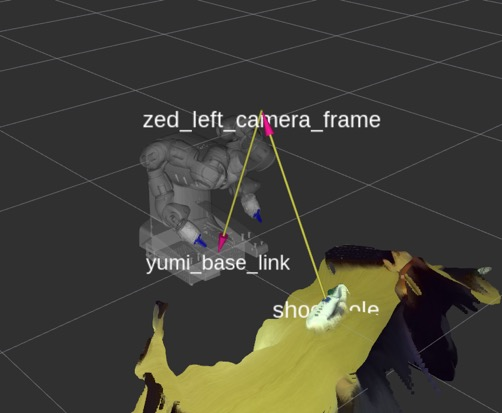
\includegraphics[height=7cm,keepaspectratio]{Implementation/cv/3dpos.jpg} \label{3dpos}}
\caption{Example of shoe hole 3D location estimation using ZED Mini}
\end{figure}

Once the 2D pixel position is computed, same approach as in Section \ref{shoeadjust} will be used to obtain its 3D real-world location $shoe\_hole$ referenced to camera frame. Related code can be found in !!!!!!. To improve its stability, 10 readings of $shoe\_hole$ will be recorded and averaged before publishing to $TF$. Figure \ref{3dpos} is the example visualized in Rviz.

\section{3D Orientation of Shoe Hole} \label{3DOrientationofShoeHole}
Due to the fact that the surrounding area of the shoe hole can be regarded as a plane, as shown in Figure \ref{plane}, its 3D orientation is the same as that of the plane. In addition, the orientation of a plane can be obtained from its plane equation. For a plane $Ax + By + Cz = D$, its normal vector is $n = Ai + Bj + Ck$.

To achieve the shoelace insertion task, a pre-insertion point called $pre\_put$ need to be defined along the normal vector direction. With this, YuMi will move its gripper to this location, then align the gripper with the normal vector, and finally move to $shoe\_hole$. After insertion, it will follow the previous path and return to $pre\_put$.

\begin{figure}[H]
\centering
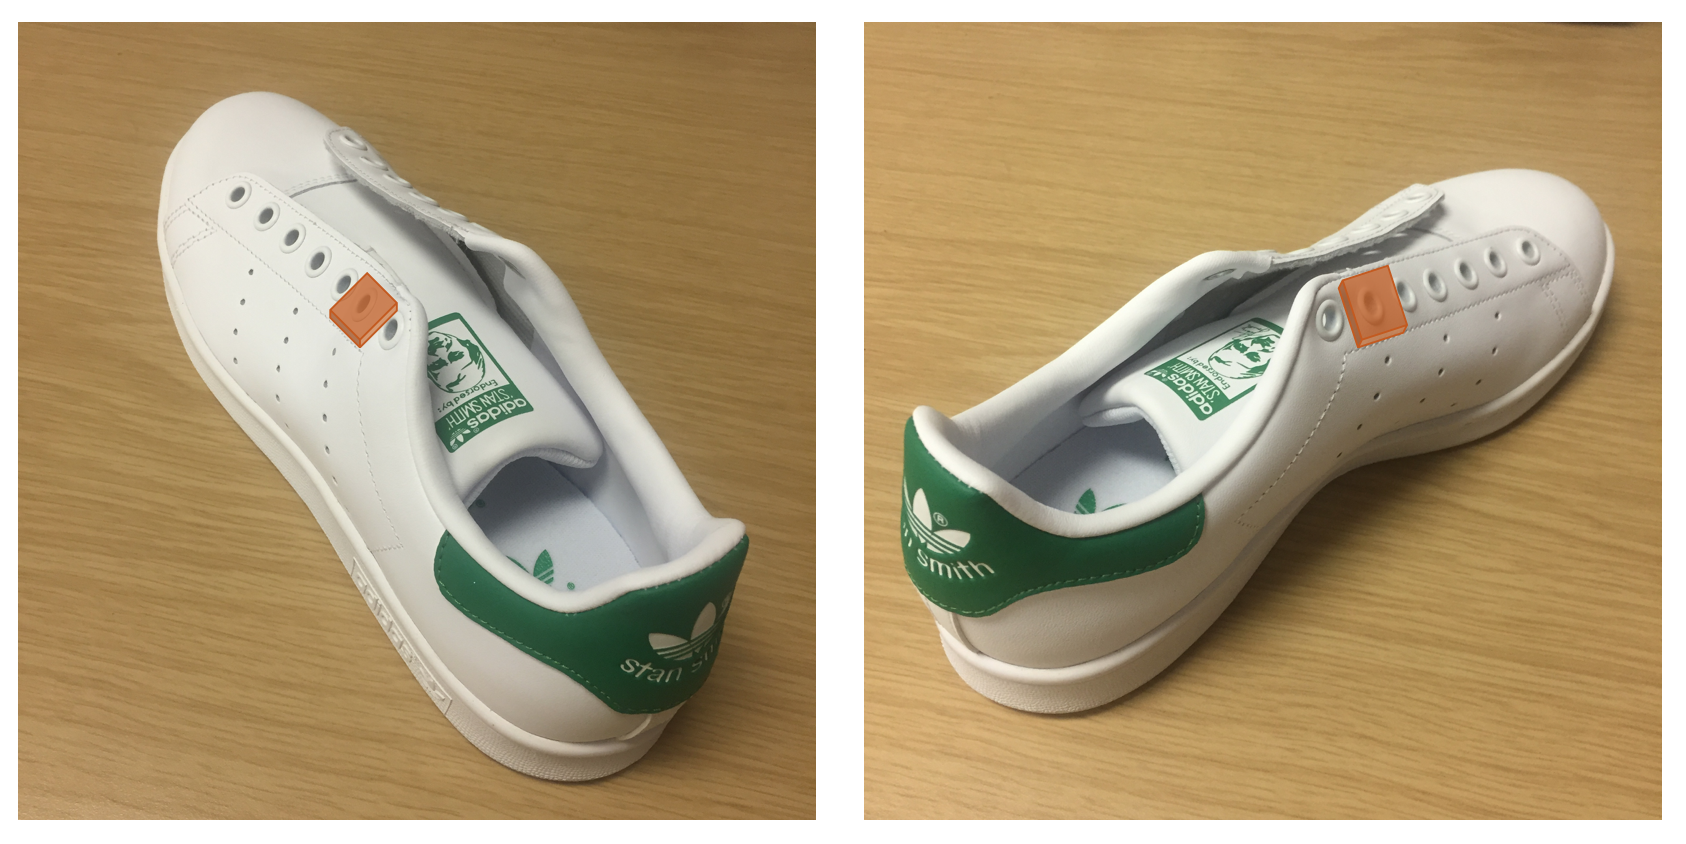
\includegraphics[width = 0.7\columnwidth]{Implementation/cv/plane.png}
\caption{The surrounding area of the shoe hole. The orientation of the orange plane is approximately same as that of the shoe hole within it.}
\label{plane}
\end{figure}

As mentioned in Background Chapter, by extracting all the surrounding point clouds of the shoe hole, RANSAC can then be applied to estimate the plane parameters A, B, C, and D, while ignoring the outliers. Here, the reasonable surrounding area is the contour area detected in Section \ref{3dlocationestimation}. In other words, it consists of all the white points in the final mask image shown in Figure \ref{zedfilter}. For ASUS Xtion camera, these points need to be converted to YuMi's axis format as before. Taking these points as input, following settings are used for RANSAC. Notice that the number of hypothetical inliers is different for these two cameras due to their different resolutions.

\begin{table}[H]
\centering
\resizebox{\columnwidth}{!}{
\begin{tabular}{||c||c|c|c||}
\hline
Camera & Number of hypothetical inliers & Distance threshold & Max iterations \\ \hline\hline
ASUS Xtion & 20 & 0.01 & 200 \\ \hline
ZED Mini 720p & 60 & 0.01 & 200 \\ \hline
ZED Mini 1080p & 300 & 0.01 & 200 \\ \hline
\end{tabular}
}
\caption{RANSAC parameters setting}
\label{ransacsetting}
\end{table}

Again, the output plane parameters are referenced to the camera frame, whose direction points into the shoe. Therefore, location $pre\_put$ can be represented as $(-0.1*A, -0.1*B, -0.1*C)$ referenced to $shoe\_hole$. The minus sign is for converting the normal vector direction to face away from the hole, $0.1$ is used to adjust the length between $pre\_put$ and $shoe\_hole$.

Another issue of this approach is that $pre\_put$ has volatility, especially for low resolution camera like ASUS Xtion. The readings fluctuate every time, which are extremely unstable. To tackle this, I firstly introduced a constraint. Since the orientation of the shoe hole is supposed to toward camera side, the x coordinate of $pre\_put$ must be smaller or equal to that of the $shoe\_hole$ (x-axis is the red line in Figure \ref{xaxis}). Therefore, the algorithm will ignore any calculated vector with unreasonable x coordinates. 

\begin{figure}[H]
\centering
\subfigure[Real-world shoe placement]{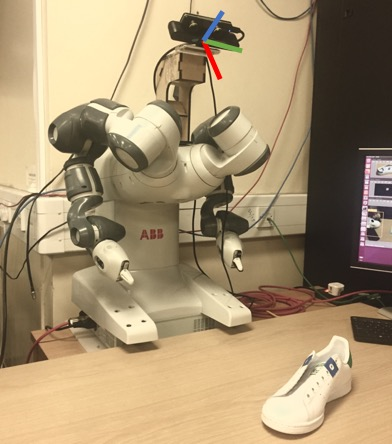
\includegraphics[height=7cm,keepaspectratio]{Implementation/cv/3dposwa.jpg} \label{xaxis}}
\subfigure[The frame relationships in Rviz]{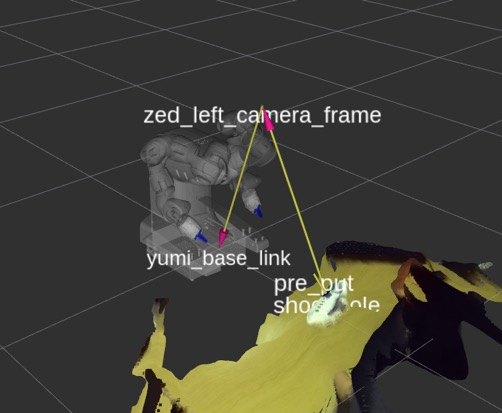
\includegraphics[height=7cm,keepaspectratio]{Implementation/cv/3dori.jpg}\label{3dori}}
\caption{Example of shoe hole 3D orientation estimation using ZED Mini}
\end{figure}

To further improve the stability and accuracy of the results, every 50 vector coefficients will be recorded when using ASUS Xtion, every 10 vector coefficients will be documented if using ZED Mini, and further data processing will be performed. The following two techniques have been experimented.

\begin{itemize}
    \item \textbf{K-means Clustering:} K-means can partition these $pre\_put$ into k clusters where each point belongs to the cluster with the nearest mean. The cluster with the most number of points will be treated as the correct one and the cluster mean is the final $pre\_put$s. However, for this approach, the number of cluster need to be defined at first. Different settings give very different results even under same environments. Once the selected cluster is wrong, the resulting point can be ridiculous sometimes, which is unreliable.
    
    \item \textbf{Average:} Considering the majority of calculated points are reliable, averaging these 50 $pre\_put$ should give a reasonable answer. This method has been experimented and proven to be effective.
\end{itemize}

The final $pre\_put$ are then be published to $TF$ topic as a transform from frame $shoe\_hole$. Figure \ref{3dori} illustrates all the frames used up to this stage.

%\section{3D Orientation of Shoelace}